%%%%%%%%%%%%%%%%%%%%%%%%%%%%%%%%%%%%%%%%%
% Beamer Presentation
% LaTeX Template
% Version 1.0 (10/11/12)
%
% This template has been downloaded from:
% http://www.LaTeXTemplates.com
%
% License:
% CC BY-NC-SA 3.0 (http://creativecommons.org/licenses/by-nc-sa/3.0/)
%
%%%%%%%%%%%%%%%%%%%%%%%%%%%%%%%%%%%%%%%%%

%----------------------------------------------------------------------------------------
%	PACKAGES AND THEMES
%----------------------------------------------------------------------------------------

\documentclass{beamer}

\mode<presentation> {

% The Beamer class comes with a number of default slide themes
% which change the colors and layouts of slides. Below this is a list
% of all the themes, uncomment each in turn to see what they look like.

%\usetheme{default}
%\usetheme{AnnArbor}
%\usetheme{Antibes}
%\usetheme{Bergen}
%\usetheme{Berkeley}
%\usetheme{Berlin}
%\usetheme{Boadilla}
%\usetheme{CambridgeUS}
%\usetheme{Copenhagen}
%\usetheme{Darmstadt}
%\usetheme{Dresden}
%\usetheme{Frankfurt}
%\usetheme{Goettingen}
%\usetheme{Hannover}
%\usetheme{Ilmenau}
%\usetheme{JuanLesPins}
%\usetheme{Luebeck}
\usetheme{Madrid}
%\usetheme{Malmoe}
%\usetheme{Marburg}
%\usetheme{Montpellier}
%\usetheme{PaloAlto}
%\usetheme{Pittsburgh}
%\usetheme{Rochester}
%\usetheme{Singapore}
%\usetheme{Szeged}
%\usetheme{Warsaw}

% As well as themes, the Beamer class has a number of color themes
% for any slide theme. Uncomment each of these in turn to see how it
% changes the colors of your current slide theme.

%\usecolortheme{albatross}
%\usecolortheme{beaver}
%\usecolortheme{beetle}
%\usecolortheme{crane}
%\usecolortheme{dolphin}
%\usecolortheme{dove}
%\usecolortheme{fly}
%\usecolortheme{lily}
%\usecolortheme{orchid}
%\usecolortheme{rose}
%\usecolortheme{seagull}
%\usecolortheme{seahorse}
%\usecolortheme{whale}
%\usecolortheme{wolverine}

%\setbeamertemplate{footline} % To remove the footer line in all slides uncomment this line
%\setbeamertemplate{footline}[page number] % To replace the footer line in all slides with a simple slide count uncomment this line

%\setbeamertemplate{navigation symbols}{} % To remove the navigation symbols from the bottom of all slides uncomment this line
}

\usepackage{graphicx} % Allows including images
\usepackage{booktabs} % Allows the use of \toprule, \midrule and \bottomrule in tables
\usepackage{listings}
\usepackage{amsmath}
\usepackage{algpseudocode,algorithm,algorithmicx}

\lstdefinestyle{customjava}{
  breaklines=true,
  frame=L,
  xleftmargin=\parindent,
  language=Java,
  showstringspaces=false,
  basicstyle=\footnotesize\ttfamily,
  keywordstyle=\bfseries\color{green!40!black},
  commentstyle=\itshape\color{gray!40!black},
  identifierstyle=\color{blue},
  stringstyle=\color{orange},
}

\lstdefinestyle{customcpp}{
  breaklines=true,
  frame=L,
  xleftmargin=\parindent,
  language=C++,
  showstringspaces=false,
  basicstyle=\footnotesize\ttfamily,
  keywordstyle=\bfseries\color{green!40!black},
  commentstyle=\itshape\color{gray!40!black},
  identifierstyle=\color{blue},
  stringstyle=\color{orange},
}
%----------------------------------------------------------------------------------------
%	TITLE PAGE
%----------------------------------------------------------------------------------------

\title[File Systems]{File Systems} % The short title appears at the bottom of every slide, the full title is only on the title page

\author{Jonathan Windle} % Your name
\institute[UEA] % Your institution as it will appear on the bottom of every slide, may be shorthand to save space
{
University of East Anglia \\ % Your institution for the title page
\medskip
\textit{J.Windle@uea.ac.uk} % Your email address
}
\date{\today} % Date, can be changed to a custom date

\begin{document}

\begin{frame}
\titlepage % Print the title page as the first slide
\end{frame}

\begin{frame}[allowframebreaks]
\frametitle{Overview} % Table of contents slide, comment this block out to remove it
\tableofcontents % Throughout your presentation, if you choose to use \section{} and \subsection{} commands, these will automatically be printed on this slide as an overview of your presentation
\end{frame}

%-------------------------------------------------------------------
\section{File System Requirements}
\begin{frame}
\frametitle{File System Requirements}
\begin{itemize}
\item Ease of use for users
\item Reliability
\item Provide a common interface to numerous technologies
\item Good performance (throughput/response time)
\item Security (esp. for multi-user/networked systems)
\item Ability to create/modify files
\item Ability to manipulate file system structure
\item Provide long term storage for user data
\begin{itemize}
\item File system must be durable, files should not disappear
\item Robust to system crashes, error free r/w
\end{itemize}
\item Ensure data is protected from invalid access, viruses, other users.
\end{itemize}
\end{frame}
%-------------------------------------------------------------------
\section{Definition}
\begin{frame}
\frametitle{Definition}
\begin{itemize}
\item File system is an OS layer that maps the blocks of data on the disk into files and directories
\item Allows blocks to be allocated to files (file creation)
\item Allows blocks to be specified by name (reference)
\end{itemize}
\end{frame}
%----------------------------------------------------------------
\section{Data Hierarchy}
\begin{frame}
\frametitle{Data Hierarchy}
\begin{itemize}
\item Lowest level stores sequences of bits: 1's and 0's
\item Collections of bytes form words
\item Word length depends on CPU architecture
\item Characters are a mapping of bytes to symbols
\item Fields are groups of characters
\item Records are groups of fields
\item Files are groups of records
\item Volume is unit of storage for files
\end{itemize}
\end{frame}
%----------------------------------------------------------------
\section{File System}
\begin{frame}
\frametitle{File System}
\begin{itemize}
\item Provides support for acting on files as a whole
\begin{itemize}
\item Opening, closing, creating, deleting and copying
\end{itemize}
\item Provides support for accessing data within a file
\begin{itemize}
\item Reading, writing, modifying, insert and delete file
\end{itemize}
\item Maintains important file characteristics
\begin{itemize}
\item Location, permission, type, access and creaation times 
\end{itemize}
\item Location is both logical and physical
\begin{itemize}
\item Logical location is user view of file
\item Physical location is actual location on disk
\end{itemize}
\end{itemize}
\end{frame}
%-------------------------------------------------------------------
\section{Directories}
\begin{frame}
\frametitle{Directories}
\begin{itemize}
\item Users view: Directories are containers for files/sub-directories
\item File system view: Directories are files; rather than user data, store information about other files etc.
\item Most file systems are hierarchial.
\end{itemize}
\end{frame}
%------------------------------------------------------------------
\section{Links}
\begin{frame}
\begin{itemize}
\item Symbolic/Soft links:
\begin{itemize}
\item Directory entry containing pathname to linked file
\item Breaks if file is moved or renamed
\end{itemize}
\item Hard links:
\begin{itemize}
\item Directory entry containing a physical block number
\item Can become invalid if physical location is changed
\item Unaffected by moving the logical location of the file
\end{itemize}
\end{itemize}
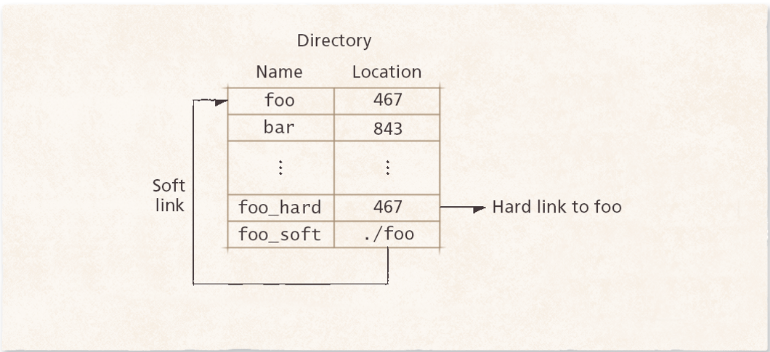
\includegraphics[scale=0.35]{links.png}
\end{frame}
%----------------------------------------------------------------
\section{File Allocation Schemes}
\begin{frame}
\frametitle{File Allocation Schemes}
\begin{itemize}
\item Main idea behind allocaation is effective utilization of file space and fast access of the files
\item Three types:
\begin{itemize}
\item Contiguous allocation
\item Linked allocation
\item Indexed allocation
\end{itemize}
\end{itemize}
\end{frame}
%-----------------------------------------------------------------
\subsection{Contiguous Allocation}
\begin{frame}
\frametitle{Contiguous Allocation}
\begin{itemize}
\item Each file has to occupy contiguous blocks on disk
\item The location of a file is defined by the disk address of the first block
\item Stores file data at contiguous address on the device.
\item Successive logical records are physically adjacent
\item Provides fast access to data
\item Leads to fragmented file system (like memory)
\item Suffficient contiguous space needed to create the file
\item Best suited to write-once media (e.g. DVDs)
\end{itemize}
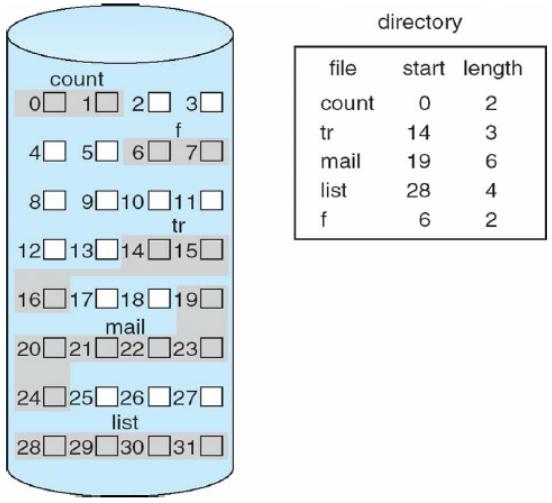
\includegraphics[scale=0.2]{contig.png}
\end{frame}
%-------------------------------------------------------------------
\subsection{Linked-List File Allocation}
\begin{frame}
\frametitle{Linked-List File Allocation}
\begin{itemize}
\item Each file is a linked list of data "chunks"
\begin{itemize}
\item Could be linked at sector level, or block level
\item Sector level provides finer grained segmentation
\item Block level provides fast access, but suffers internal fragmentation
\end{itemize}
\item Files can be easily grown:
\begin{itemize}
\item There is no external fragmentation with linked allocation
\item Performance might be an issue
\end{itemize}
\item Only supports sequential access:
\begin{itemize}
\item Need to traverse the linked list to locate particular segments	
\end{itemize}
\end{itemize}
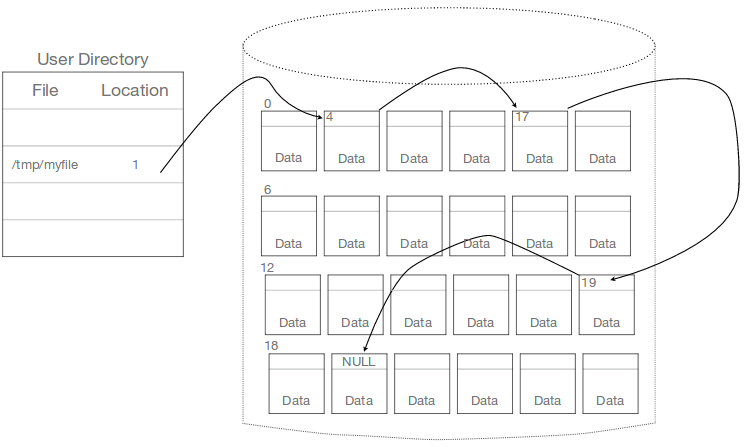
\includegraphics[scale=0.2]{linked.png}
\end{frame}
%---------------------------------------------------------------------
\subsection{File Allocation Table (FAT)}
\begin{frame}
\frametitle{File Allocation Table (FAT)}
\begin{columns}[c]
\column{.45\textwidth}
\begin{itemize}
\tiny
\item File stores reference into a block allocation table called the FAT
\item Like linked allocation, exceoot don't keep the links in the blocks themselves, use FAT instead:
\begin{itemize}
\tiny
\item Each FAT entry is a disk sector or number
\item Special values for ``last block in file" and ``free block"
\end{itemize}
\item FAT stored on disk but cached when file system is mounted
\item Can support random access to files
\item Originally each FAT enter was 16 bits:
\begin{itemize}
\tiny
\item Unsustainable for large disks
\item Problem addressed by FAT32 standard
\end{itemize}
\end{itemize}
\column{.45\textwidth}
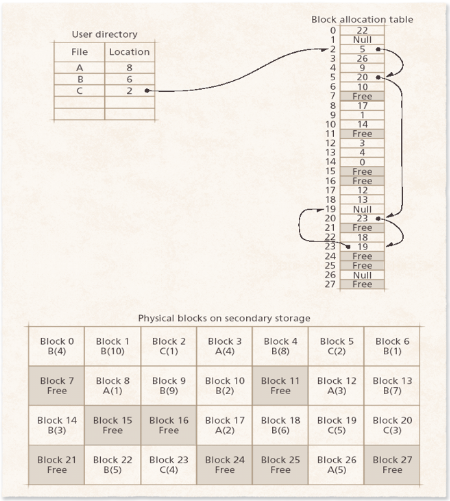
\includegraphics[scale=0.35]{fat.png}
\end{columns}
\end{frame}
%-------------------------------------------------------------------
\subsection{Indexed File Allocation}
\begin{frame}[allowframebreaks]
\frametitle{Indexed File Allocation}
\begin{itemize}
\item Supports random accesses by bringing pointers to blocks together into an index block
\item Allocate block pointers contiguously in metadata (index block) when file is created
\item Files can be easily grown within limit of index block size
\item Allocate blocks on demand by filling in the pointers dynamically as file is written
\item When applying this strategy, acccessing any place on the disk requires no more than two disk operations, one to acccess the index block, one to acces the data.
\item But the size of the file is limited. For example, if disk blocks have 4kB and the block number occupies 32 bytes, the maximum size of the file is 1024$\times$4kB = 4MB.
\item This constraint is addressed by Linked-Indexed and Multilevel-Indexed File allocation schemes.
\end{itemize}
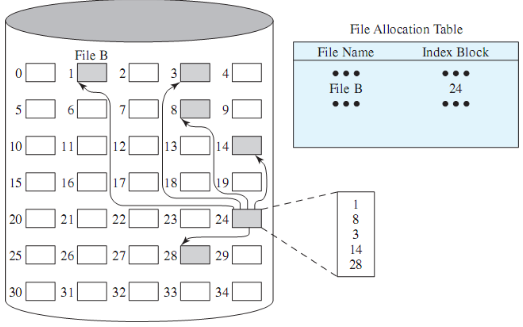
\includegraphics[scale=0.5]{index.png}
\end{frame}
%-----------------------------------------------------------------
\subsection{Linked-Indexed Allocation}
\begin{frame}
\frametitle{Linked-Indexed Allocation}
\begin{itemize}
\item A combination of linked and index approaches
\item The numbers of consecutive disk blocks with the file contents are gathered in the index block.
\item A file is identified by the number of the first index block
\item If the numebr of blocks creating the files doesn't fit into one index block, the last number in this block points to the next index block.
\item For example - if the disk blocks have 4kB and the block number has 32 bytes, then one index block can contain 1023 block numbers with file contents and one number of following index block. IF we have a 42MB file, then we'll also have 11 index blocks. Access to data fragments at the end of the file may require 12 disk operations
\end{itemize}
\end{frame}
%------------------------------------------------------------------
\subsection{Multilevel-Indexed File Allocation}
\begin{frame}
\frametitle{Multilevel-Indexed File Allocation}
\begin{itemize}
\item Multilevel index allocation means that index blocks with disk blocks containing file contents create a tree of a specific depth
\item For example, in the two-level indexing, the main index block (first level) contains the numbers of index blocks of the second level, which in turn contain the number of blocks constituting the file contents.
\item For example, if the disk blocks have 4kB and block number occupies 32 bytes, then with two-level indexing the size of files is limited to 4GB and with third level indexing it is limited to 4TB.
\end{itemize}
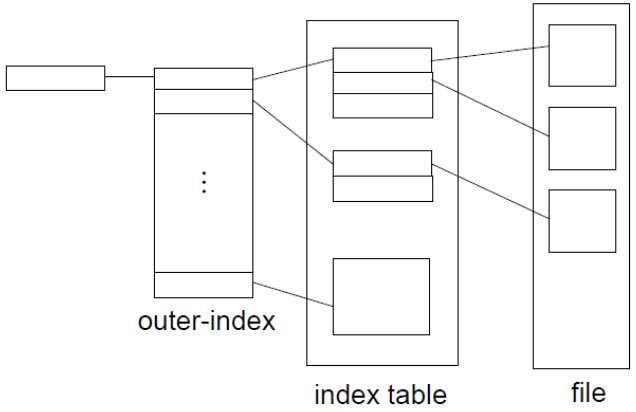
\includegraphics[scale=0.25]{multi.png}
\end{frame}
%-----------------------------------------------------------------
\subsection{UNIX - inodes}
\begin{frame}[allowframebreaks]
\frametitle{UNIX - inodes}
\begin{itemize}
\item In the UNIX system files are represented by so called inodes
\item One inode for each
\item An inode contains an index of disk block numbers
\item The first 10 are the numbers of the first 13 file contents blocks
\item The eleventh number is a number of the index block (first level) to the next file blocks
\item The last number is the nuumber of the third level index block of following file blocks
\item Thanks to this approach, the number of disk operations required to access any place in the file depends on the file size and oscillates between 1 and 4.
\end{itemize}
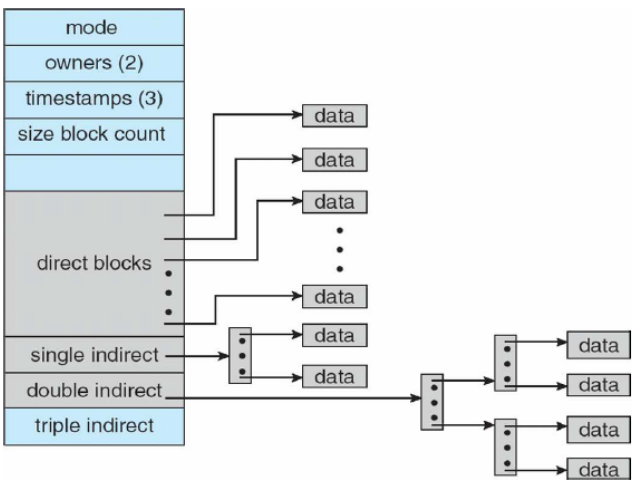
\includegraphics[scale=0.45]{inodes.png}
\end{frame}
%-----------------------------------------------------------------
\subsection{Managing Free Space}
\begin{frame}
\frametitle{Managing Free Space}
\begin{itemize}
\item Not all blocks are occupied.
\item There has to be a way of storing informaaation concerning empty blocks
\item Two methods considered:
\begin{itemize}
\item Maintaining a list of empty blocks
\item Maintaining a bitmap image of blocks
\end{itemize}
\end{itemize}
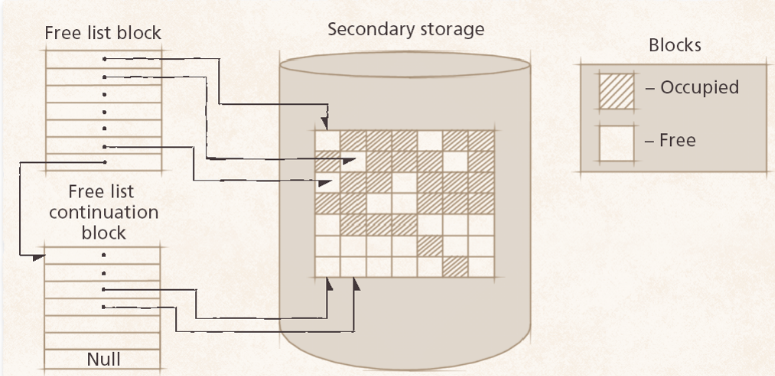
\includegraphics[scale=0.225]{flist.png}
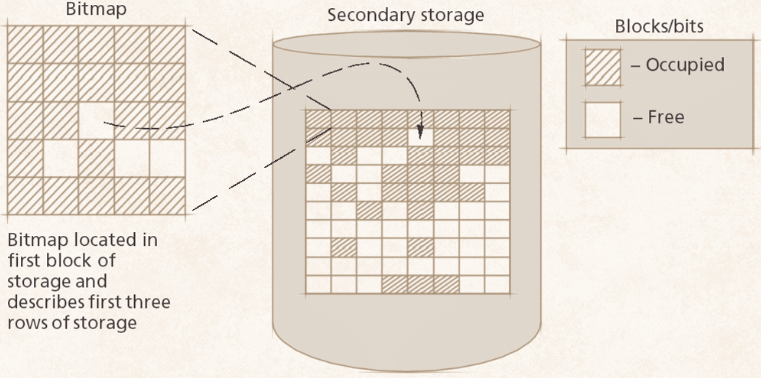
\includegraphics[scale=0.225]{fbit.png}
\end{frame}
%------------------------------------------------------------------

\begin{frame} 
\Huge{\centerline{The End}}
\end{frame}

\end{document}